 \section{Visual Studio Code} \label{vscode} \index{Visual~Studio~Code}
 
 \textbf{Visual Studio Code} (zkráceně VS Code) je pokročilý textový editor od Microsoftu, speciálně navržený pro programátory čehokoliv.
 Jde o~program, který toho hodně umí sám a ještě mnohem víc se toho může naučit, pokud do něj doinstalujeme další rozšíření, 
 tzv.~\textbf{pluginy}, \index{plugin}
 například  \hyperref[platformio]{PlatformIO}, což je plugin speciálně zaměřený na programování \hyperref[cip]{čipů}. 
% V této kapitole se zaměříme na na programování 
 
 \subsubsection*{Postup}
 
 Pokud s~programováním čipů začínáme, čekají nás tyto úkoly:
 \begin{enumerate}
 	\item  nainstalovat prostředí {\it Visual Studio Code}
 	\item  do Visual Studio Code nainstalovat doplněk {\it PlatformIO }
 	\item  přes PlatformIO založit nový projekt
 	\item  napsat zdrojový kód, přeložit a~dostat jej do čipu 
 \end{enumerate}
 Toto vše podrobněji probereme na dalších řádcích. 
 
 \label{vsc} \subsection{Nainstalujte  Visual Studio Code} 
 
 Instalujte podobně jako každý jiný program, stahujte zde: \url{https://code.visualstudio.com/}  
 
 \textbf{POZOR:} Pokud jméno vašeho uživatelského účtu na PC obsahuje diakritiku (čárky, háčky), speciální znaky (znaky mimo \href{https://cs.wikipedia.org/wiki/ASCII}{ASCII} tabulku) nebo i~mezery, můžete mít problémy s~používáním PlatformIO.
 
 Prakticky jediné funkční řešení tohoto problému je vytvořit si na PC nový uživatelský účet a používat ho pro práci s \textbf{VS Code} a \textbf{PlatformIO}. 
 
 
 \subsubsection{Nainstalujte PlatformIO} \label{platformio}
 
 \index{PlatformIO} \textbf{PlatformIO} (zkráceně PIO) je ten software, který umožní program v~C++ 
 přeložit tak, aby ho čip pochopil a~taky ho do čipu umí nahrát. 
 Instalace podle návodu zde: \url{http://docs.platformio.org/en/latest/ide/vscode.html#installation}
 
 \label{vsc:newproject} \subsubsection{Založte nový projekt}
 
 Program (ne)píšete jen do jednoho souboru, ale aby vše fungovalo, potřebujete vícero dalších souborů, které dohromady tvoří tzv. {\bf projekt}\index{projekt}.
 Tyto soubory jsou mezi sebou hodně provázané, takže v případě přesunu projektu například z kroužku domů je potřeba zkopírovat celý adresář projektu. 
 %todo ověřit 

%  a~navíc vázané na konkrétní místo uložení, 
% takže vám po překopírování na jiný počítač pravděpodobně program nepůjde přeložit a~nebo 
% nahrát do čipu. Řešení: \fxnote*[author=JP]{Opravdu jsou s tím pořád tak velké problémy? Nestačí si prostě uložit (flash disk, mail, Google Drive)/zaverzovat (Git) celou složku s projektem a fungovat?}{uložit celý projekt na flash disk}. 
% Na novém počítači založit nový projekt a~potřebné části zdrojového kódu kopírovat pomocí {\it Ctrl+C}, {\it Ctrl+V}. 
 
 
 
 \begin{enumerate}
 	\item Založte nový projekt z~ikonky \uv{domeček} -- viz \url{http://docs.platformio.org/en/latest/ide/vscode.html#quick-start}.
 	\item Do kolonky {\it Board} se musí vybrat správná deska.
 		Desek je přes 400 a~jsou rozdělené do sekcí řazených podle abecedy vyznačených šedivou barvou.
 		Vám ale stačí kliknout na kolonku Board a na klávesnici napsat:
 		\begin{enumerate}
 			\item {\it Espressif ESP32 Dev Module} a vybrat tuto desku, pokud používáte samotnou vývojovou desku ESP32 DevKitC s modulem ESP32-WROOM32
 			\item {\it \href{https://docs.platformio.org/en/latest/boards/espressif32/alksesp32.html}{ALKS ESP32}} a vybrat tuto desku, pokud využíváte výukový kit ALKS (viz sekce \ref{alks}) 
 		\end{enumerate}
 	Kolonka {\it Framework } se potom vyplní automaticky. 
 	\item  Zbývá vybrat adresář, do kterého bude projekt uložen.
 	Tento adresář si předem vytvořte, s~adresářem vytvářeným za pochodu má VS Code kdovíproč problém.
 	Odškrtněte zatržítko {\it Use defalut folder} a~zvolte vámi vytvořený adresář. Pokud si zapomenete nastav vlastní složku pro projekt, PIO projekt vytvoří někde v rámci složky Dokumenty. Nejjednodušší je vytvořit znovu nový projekt.
 \end{enumerate}
 
 Pro Linux Lubuntu: projekt musí být uložen na pevném disku, ne na flešce, jinak prostě nepojede, netuším proč.  
 
 \subsubsection{Napiště zdrojový kód, přeložte jej a~nahrejte jej do čipu}
 
 \begin{figure}[h]
 	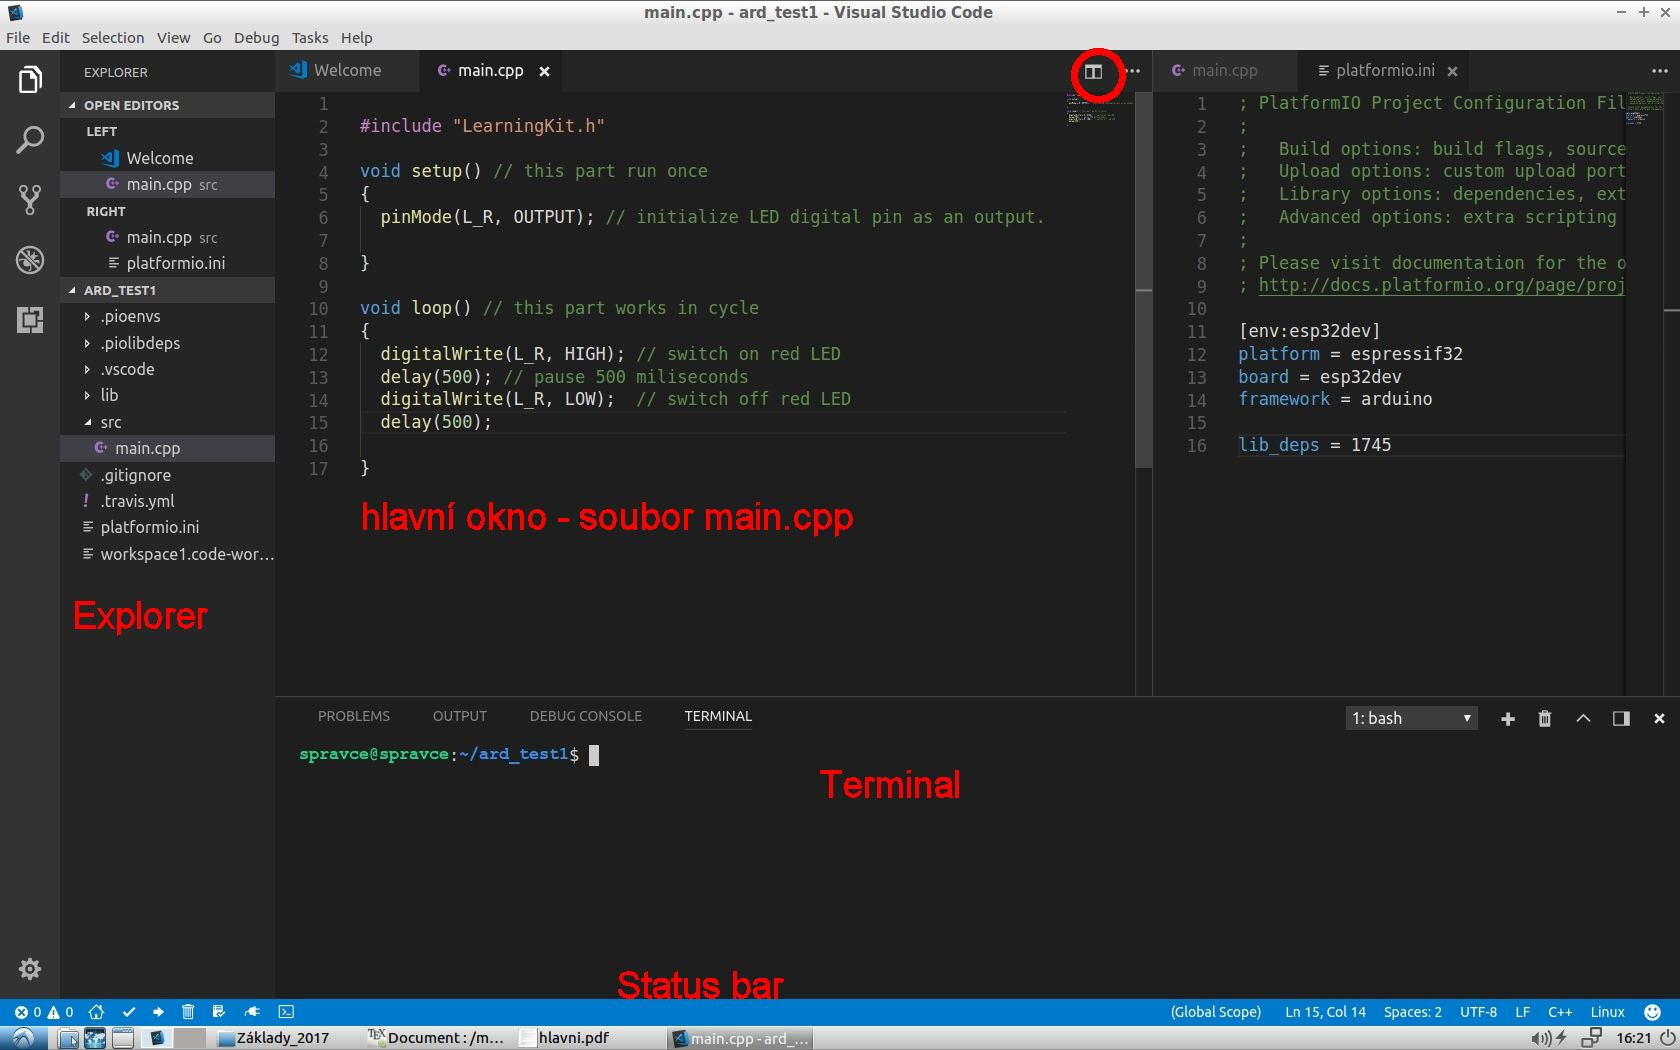
\includegraphics[width=\textwidth]{soubory/rozlozeni2.jpg}
 	\caption{Rozložení oken v~programu {\it VS Code}} 
 	\label{fig:vsc_rozlozeni}
 \end{figure}	
 
 \hypertarget{explorer}{}
 Obrázek \ref{fig:vsc_rozlozeni} na straně~\pageref{fig:vsc_rozlozeni} ukazuje rozložení oken v~rámci projektu.
 Hlavní okno  rozdělte na dvě části pro zobrazení dvou upravovaných souborů pomocí ikony v~kroužku.
 Začínáme v~okně {\bf Explorer}, \index{Explorer}
 kde je umístěna adresářová struktura projektu\footnote{Pokud toto okno není vidět, zobrazíte ho v~menu {\it View} položka {\it Explorer} }.
 Otevřete soubory {\it platformio.ini} a~v~adresáři {\it src} soubor {\it main.cpp}. 
 
 Pro pohodlnou práci s~deskou \hyperref[alks]{ALKS} byla napsaná tzv. knihovna {\it ArduinoLearningKitStarter}. 
 Aby fungovala, musí být do souboru {\it platformio.ini} dopsán řádek {\tt lib\_deps = 1745} (bez mezery na začátku řádku) a~do záhlaví souboru {\it main.cpp} doplňte
 % {\tt include "LearningKit.h\"}.  
 %% nahrazeno \verb| include "LearningKit.h"|
 \verb| include "ALKS.h"|
 Dále dopište do souboru {\it main.cpp} kód, který bliká červenou LED.
 Vše je vidět na obrázku \ref{fig:vsc_rozlozeni}.
 Celý zdrojový kód tohoto prvního programu (obsah souboru {\it main.cpp}) je uveden v~kapitole \ref{cpppr1}.
 
 Teď budou potřeba další dvě části VS Code: terminál \index{terminál} (okno vpravo dole) a~stavový řádek (Status~bar\index{Status~bar} -- proužek pod terminálem). 
 Na stavovém řádku klikněte na ikonu šipky\footnote{totéž provede {\it Ctrl+Alt+U}} (pátá zprava) a~{\it PlatformIO} se pokusí váš program přeložit a~nahrát do čipu. 
 Pokud chcete program pouze přeložit, klikněte na ikonu zatržítko\footnote{totéž provede {\it Ctrl+Alt+B}} hned vedle. 
 
 Při prvním pokusu nahrát program do čipu na Linuxu může mít {\it PlatformIO} problém, že nenajde USB spojení na desku s~čipem a~vyžaduje ho doistalovat. 
 Zpráva\footnote{\tt Warning! Please install `99-platformio-udev.rules`} se objeví v~terminálu včetně nápovědy,\footnote{\url{https://raw.githubusercontent.com/platformio/platformio/develop/scripts/99-platformio-udev.rules}} jak to udělat.
 Nápověda je ale tak podrobná, že to středně poučený linuxový laik s~pomocí internetu zvládne.
 Při všech dalších překladech už to nebude problém.  
 
 Další programy budou uvedeny v~kapitole \ref{cpppr}. 
 
 
 
 